% Copyright (C) 2026 Steve Prud'Homme. Texte : voir LICENSE-NOTICE.md.
% Manuscrit de travail ; les figures autorisées et FITS associés sont CC0-1.0.
\documentclass[11pt,letterpaper]{article}
\usepackage[margin=2.2cm]{geometry}
\usepackage{fontspec}
\setmainfont{TeX Gyre Pagella}
\setsansfont{TeX Gyre Heros}
\usepackage[english,french]{babel}
\usepackage{microtype,graphicx,booktabs,tabularx,amsmath,caption,float,csquotes}
\usepackage[backend=biber,style=apa,sorting=nyt,sortcites=true]{biblatex}
\DeclareLanguageMapping{french}{french-apa}
% Adaptations vérifiées contre le guide UQAM-APA : « et », et al. en italique.
\DeclareDelimFormat{finalnamedelim}{\addspace et\space}
\DeclareDelimFormat[bib,biblist]{finalnamedelim}{\addspace et\space}
\DefineBibliographyExtras{french}{\protected\def\mkbibnamefamily#1{#1}}
\DefineBibliographyStrings{french}{andothers={\mkbibemph{et\addabbrvspace al\adddot}},retrieved={Récupéré},from={de}}
\makeatletter
% APA ajoute sa virgule au nom précédent ; l'enlever avant le dernier « et ».
\renewcommand*{\apablx@ifnotfinalname}{\ifboolexpr{
  test {\ifnumless{\value{listcount}}{\numexpr\value{liststop}-1\relax}} or test \ifmorenames}}
\makeatother
% Communications publiées sans direction scientifique renseignée : « Dans » + actes.
\DeclareBibliographyAlias{inbook}{uqamproceedings}
\DeclareBibliographyDriver{uqamproceedings}{%
  \usebibmacro{bibindex}\usebibmacro{begentry}\usebibmacro{author/editor}%
  \setunit{\printdelim{nametitledelim}}\newblock\usebibmacro{title}%
  \newunit\newblock\printtext{Dans\addspace}\printfield[emph]{booktitle}%
  \newunit\newblock\printlist{publisher}%
  \newunit\newblock\usebibmacro{doi+url}\usebibmacro{finentry}}
\addbibresource{references.bib}
\usepackage{xurl,xcolor}
\usepackage[colorlinks=true,linkcolor=blue!45!black,urlcolor=blue!45!black,citecolor=blue!45!black]{hyperref}
\usepackage{fancyhdr}
\pagestyle{fancy}\fancyhf{}
\fancyhead[L]{\small GNU Astrophotography Recycle}
\fancyhead[R]{\small Étude exploratoire}
\fancyfoot[C]{\thepage}
\setlength{\headheight}{14pt}
\setlength{\emergencystretch}{2em}
\captionsetup{font=small,labelfont=bf}
\graphicspath{{../images/satellites/}}
\hypersetup{pdftitle={Réidentification exploratoire de trois satellites connus dans des images du Seestar S50},pdfauthor={Steve Prud’Homme},pdflang={fr-CA}}
\title{Réidentification exploratoire de trois satellites connus dans des images archivées du Seestar S50\\[.4em]\large Une étude de science citoyenne}
\author{Steve Prud’Homme\\\small Observateur citoyen et mainteneur de GNU Astrophotography Recycle}
\date{18 novembre 2026\\\small Manuscrit de travail, non évalué par les pairs}
\begin{document}
\maketitle
\begin{abstract}
Des photographies astronomiques prises pour une cible fixe peuvent conserver des passages fortuits d’objets mobiles.
Cette étude examine seize poses Seestar S50 de dix secondes du champ d’IC 342, réparties en deux séries.
Elle demande si des traces archivées sont compatibles avec des passages de satellites connus.
Les copies sont vérifiées par empreintes. Les étoiles sont recalées vers un étalonnage céleste fourni.
Quatre traces choisies visuellement sont mesurées sur les pixels natifs, puis comparées localement à un catalogue orbital historique avec SGP4.
Trois associations sont plausibles : KUIPER-00116 (NORAD 65153), STARLINK-1301 (45361) et CENTISPACE-1 S13 (62582).
Les écarts transversaux médians sont respectivement 60,1, 33,7 et 29,7 secondes d’arc ; les écarts d’orientation restent inférieurs à 0,12 degré.
Une quatrième trace faible demeure douteuse et non identifiée.
Les 935 propositions automatiques ne constituent pas autant d’objets ; la sensibilité du détecteur n’est pas établie.
La datation UTC, la convention temporelle et la précision absolue complète restent non qualifiées.
Les données autorisées, le journal et une recette guidée sont publiés pour permettre la vérification citoyenne.
Il s’agit de passages possiblement retrouvés d’objets connus, sans identification confirmée ni découverte d’un nouveau satellite.
\end{abstract}
\noindent\textbf{Mots-clés :} science citoyenne ; Seestar S50 ; archives FITS ; satellites artificiels ; SGP4 ; reproductibilité.

\begin{otherlanguage}{english}
\section*{Abstract}
Astronomical images acquired for a fixed target may preserve incidental passages of moving objects.
This study examines sixteen ten-second Seestar S50 exposures of the IC 342 field, arranged in two series.
It asks whether archived streaks are consistent with passages of known satellites.
File hashes verify the copies. Stellar registration connects the frames to a supplied celestial calibration.
Four visually selected streaks are measured on native pixels and compared locally with a historical orbital catalogue using SGP4.
Three associations are plausible: KUIPER-00116 (NORAD 65153), STARLINK-1301 (45361), and CENTISPACE-1 S13 (62582).
Their median cross-track discrepancies are 60.1, 33.7, and 29.7 arcseconds, respectively; orientation differences remain below 0.12 degrees.
A fourth, weak feature remains doubtful and unidentified.
The 935 automated proposals do not represent 935 objects, and detector sensitivity has not been established.
UTC timing, timestamp convention, and the complete absolute error budget remain unqualified.
Authorized data, a candidate journal, and a guided reproduction recipe are released to support citizen verification.
These are possible recoveries of passages by known objects, with no confirmed identification or discovery of a new satellite.
\end{otherlanguage}
\par\smallskip
\noindent\textbf{Keywords:} citizen science; Seestar S50; FITS archives; artificial satellites; SGP4; reproducibility.

\section{Introduction et hypothèses}
Une archive photographique peut contenir des phénomènes qui ne motivaient pas l’acquisition initiale.
La question étudiée est concrète : des lignes visibles dans des poses du champ d’IC 342 correspondent-elles à des satellites catalogués ?
L’hypothèse principale est qu’un passage orbital proche dans le ciel et dans le temps explique certaines traces.
Les hypothèses concurrentes comprennent un autre satellite, un avion, un météore, un défaut du capteur et un résidu du traitement.
Une forme rectiligne seule ne distingue pas ces possibilités.

Les travaux présentés à AMOS par \textcite{rood} associent alignement stellaire, différences d’images, recherche de lignes et comparaison aux éléments orbitaux.
Ils concernent une instrumentation et une cadence différentes.
La présente étude reprend cette famille d’opérations, sans reproduire l’ensemble de leur chaîne ni transférer ses performances annoncées.
Elle ne détermine pas une nouvelle orbite et ne recherche pas exhaustivement tous les satellites.
Il s’agit d’une revue ciblée guidée, distincte de la fouille générale des archives, qui reste en pause.

\section{Données, provenance et participation citoyenne}
\subsection{Échantillon photographique}
L’échantillon comprend seize FITS individuels, de 1080 par 1920 pixels natifs, fournis par l’auteur.
Chaque durée déclarée est de dix secondes.
Les identifiants publics S03-01 à S03-08 et S04-01 à S04-08 désignent deux fenêtres déjà sélectionnées dans l’inventaire local.
Les dates déclarées vont du 20 septembre 2025 à 00:15:34,072594 à 01:30:36,238535.
La cadence est proche de cinq minutes. Elle ne permet pas de relier les trois satellites proposés comme un même objet.
Cet échantillon n’est pas représentatif de toute l’archive, des nuits ou des champs disponibles.

Les seize fichiers totalisent 66\,447\,360 octets.
Un manifeste public conserve noms d’origine, noms courts, tailles, dates et SHA-256.
Le renommage des copies ne change pas leur contenu.
Les originaux et les copies d’entrée sont lus sans réécriture ; les calculs produisent des fichiers séparés.
Le format FITS sépare pixels et métadonnées \parencite{fits}.
La présence d’une date dans un en-tête n’établit pas la justesse de l’horloge qui l’a produite.

\begin{figure}[htbp]
\centering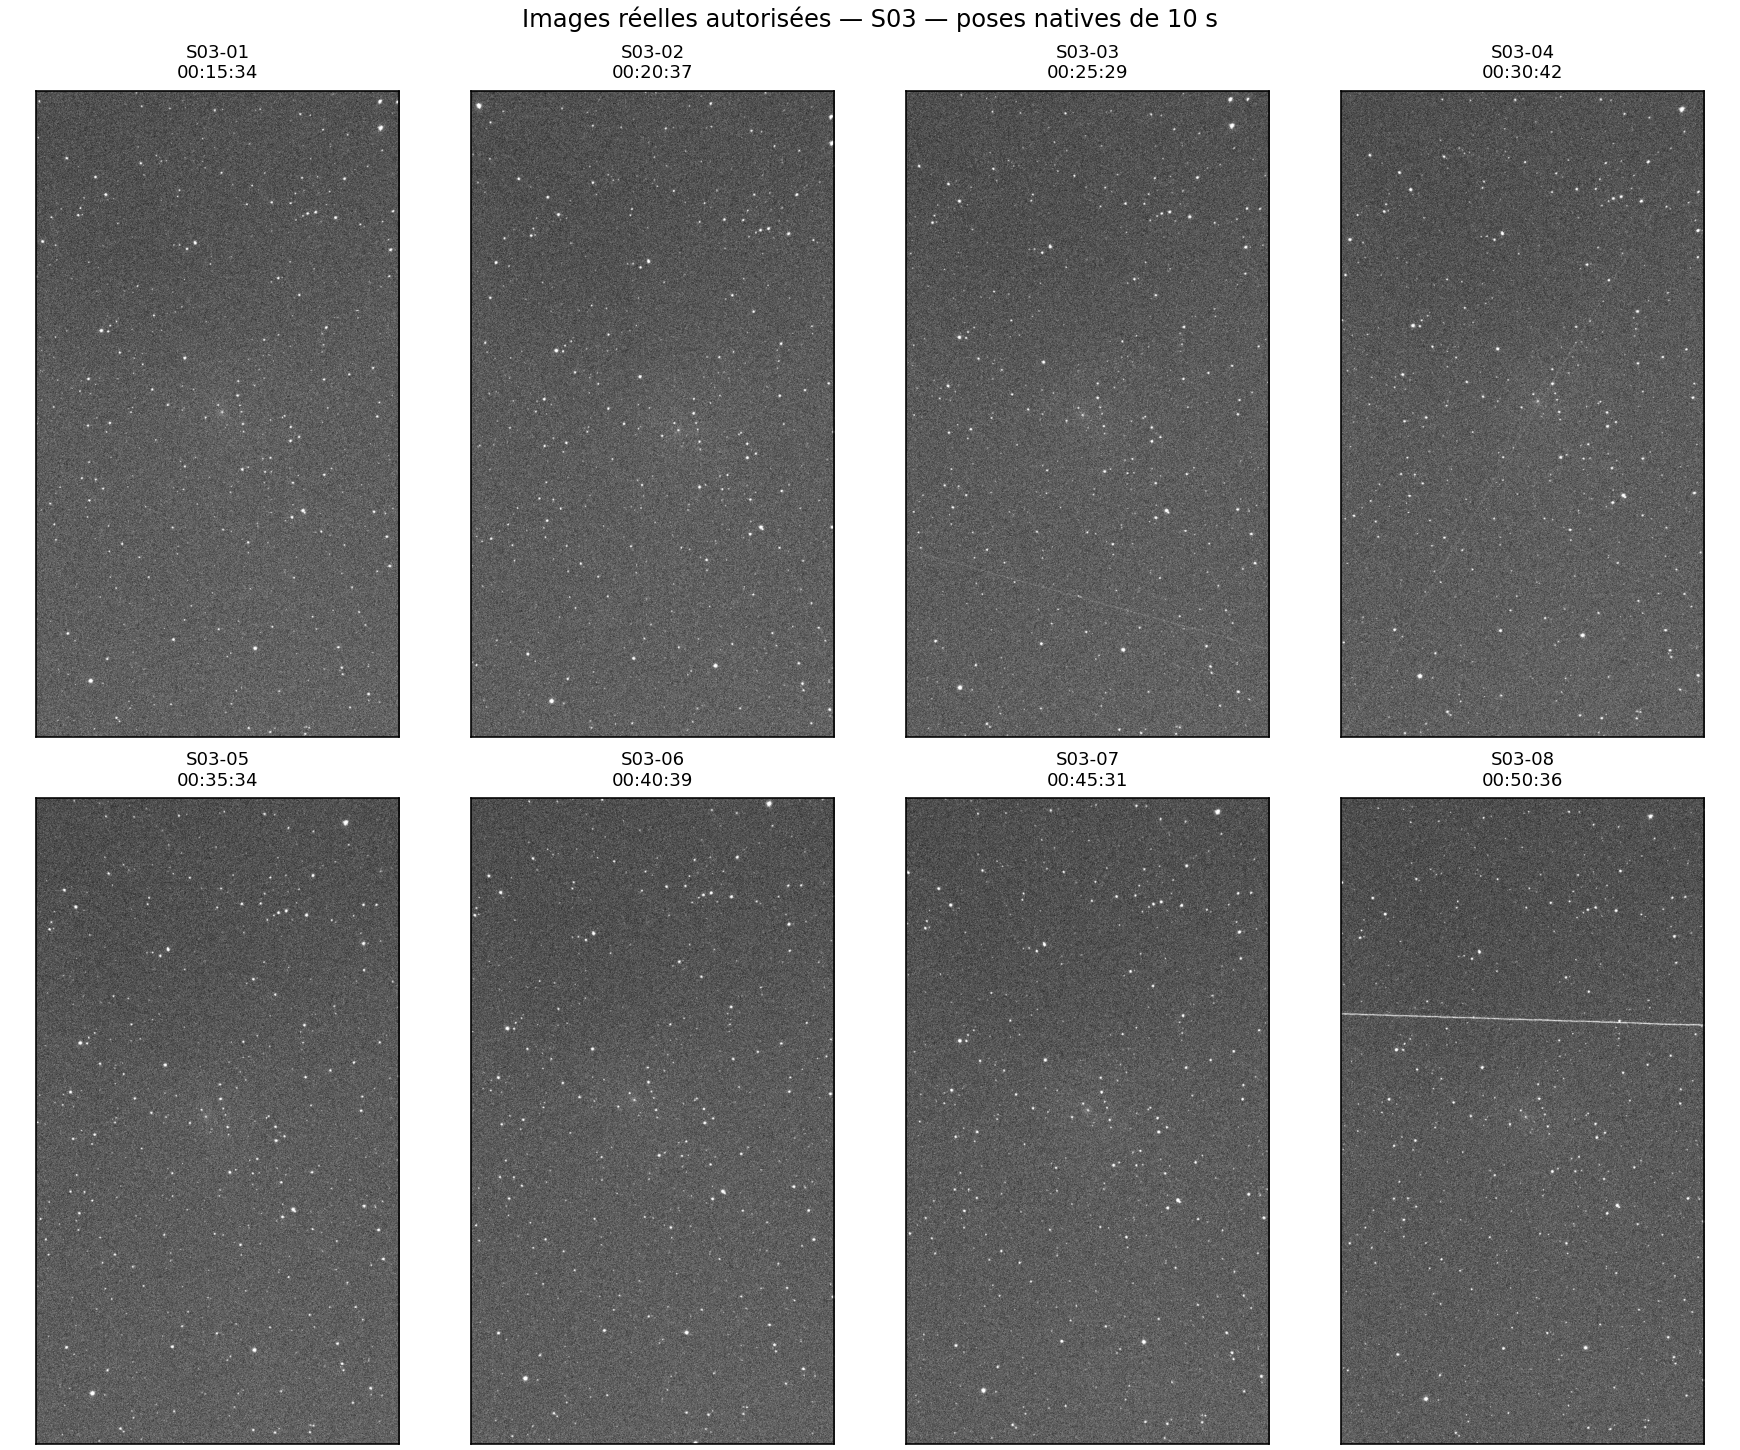
\includegraphics[width=.91\linewidth]{S03-overview.png}
\caption{Les huit poses réelles S03, ordonnées par identifiant et heure déclarée. Le contraste d’affichage est calculé par percentiles. Les pixels FITS ne sont pas réécrits. Une trace n’est pas présente dans chaque pose.}
\label{fig:overview}
\end{figure}

\subsection{Rôle citoyen et droits}
L’auteur fournit les observations et formule la question de recherche à partir de ses archives.
Il demande une méthode reproductible, un journal des hypothèses et un retour accessible à la communauté.
Ces choix s’inscrivent dans les principes de participation, de crédit et de partage des résultats décrits par l’\textcite{ecsa}.
Ils ne constituent pas une certification de conformité à ces principes.
La revue demeure limitée à un observateur et à une assistance logicielle ; aucun examen scientifique indépendant n’est revendiqué.

L’auteur déclare être membre de la Société d’Astronomie de Montréal et du Club d’Astronomie Bois de Belle-Rivière-Mirabel.
Les vocables ont été contrôlés sur leurs sites \parencite{sam,club}.
Les adhésions sont déclarées par l’auteur ; les organismes n’endossent pas cette étude par cette mention.

Le 18 novembre 2026, l’auteur a autorisé la publication des seize FITS sélectionnés et de leurs en-têtes sous CC0-1.0.
Cette décision rend publics les dates et le site inscrits, pas l’ensemble de ses archives.
Les catalogues orbitaux tiers gardent leurs propres conditions et ne sont pas redédiés au domaine public.

\section{Méthodes}
\begin{figure}[htbp]
\centering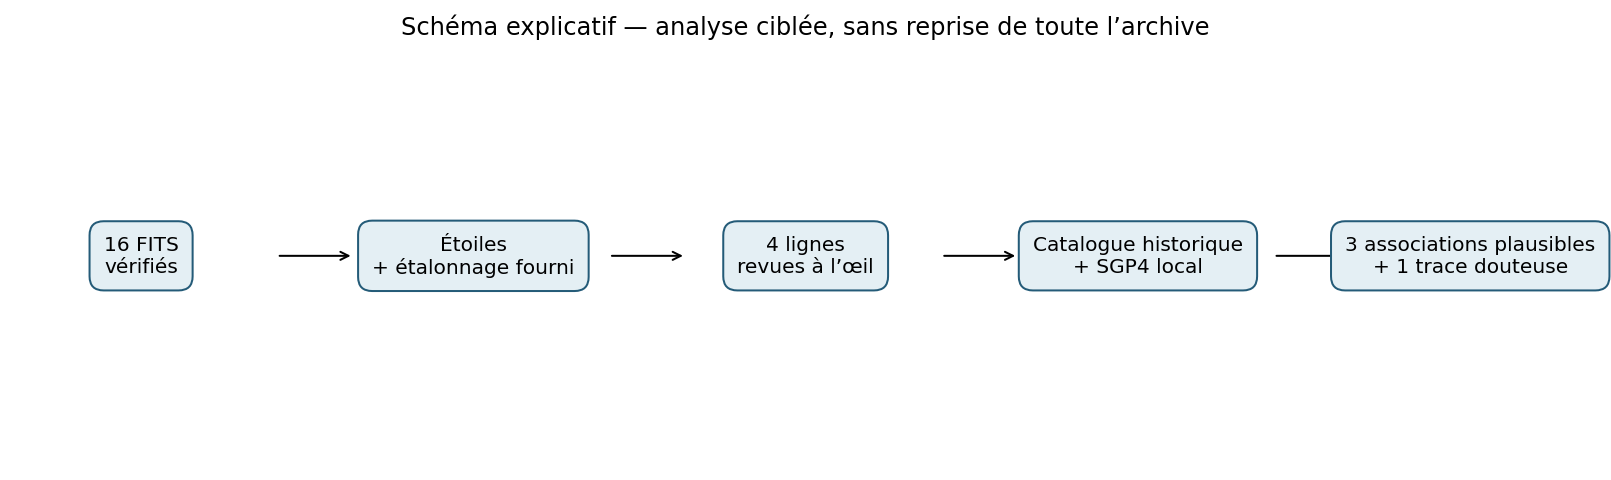
\includegraphics[width=\linewidth]{workflow.png}
\caption{Schéma explicatif du parcours ciblé. Les références célestes sont fournies. La sélection visuelle des quatre traces précède le nouveau rapprochement orbital. La comparaison aux réponses historiques vient après la recherche.}
\label{fig:workflow}
\end{figure}

\subsection{Recalage et étalonnage fourni}
Le détecteur historique extrait les centres stellaires.
Les transformations de rotation et translation entre poses utilisent les fonctions historiques, sans changement de seuil.
Des étoiles de contrôle réparties dans le champ sont réservées avant ajustement.
La première pose de chaque série conserve une transformation identité exacte.
Un ajustement inutile de cette identité introduirait des arrondis susceptibles de modifier le masque des bords rééchantillonnés.

Le passage de S04 à S03 est recalculé.
Le pont de S03-01 vers une référence antérieure est aussi recalculé, à partir de 696 centres stellaires fournis.
Le pont réserve 26 correspondances de contrôle : médiane 0,353 pixel, percentile 95 de 0,872 pixel, neuf cellules occupées sur neuf et quatre quadrants sur quatre.
Ces nombres contrôlent un recalage relatif ; ils ne constituent pas un budget d’erreur céleste absolue.

La carte WCS, avec ses termes de distorsion, est fournie dans \texttt{calibration.json}.
Elle provient d’un empilement local identifié par empreinte, qui n’est pas ajouté aux seize FITS publiés.
La recette reconstruit les transformations vers cette carte, mais ne reconstruit pas indépendamment la solution astrométrique initiale.
Cette dépendance fournie est explicite et limite la portée de la reproductibilité.
Les directions finales utilisent le repère ICRS de cette carte.

\subsection{Repérage et sélection des traces}
Pour le repérage, chaque image est réduite par moyenne de blocs de quatre par quatre pixels.
Les blocs non finis ou contenant une valeur au moins égale à 65\,000 sont masqués.
Les images sont alignées, puis la référence médiane des huit poses est soustraite.
Un complément de recherche intègre les valeurs suivant des lignes, par pas angulaire de 0,5 degré.
Il exige au moins 100 cases de support, un score robuste de 8, un lissage radial de 0,6 case et un fond gaussien de largeur 5 cases.
Le score est empirique ; il n’est pas une probabilité d’existence.
Toutes les propositions sont conservées, y compris les bords et résidus d’étoiles.

La revue visuelle initiale a retenu S03-03, S03-08, S04-01 et S04-04 avant le nouveau classement orbital.
Les points de départ sont publiés dans \texttt{review-selection.json}, sans noms de satellites.
Ce choix guidé n’est pas une évaluation aveugle de détection.
Les paramètres ne sont pas réajustés après les rapprochements.

\subsection{Mesure sur les pixels natifs}
Une ligne $y=m(x-x_c)+b$ est ajustée près de la sélection initiale.
Le fond natif est retiré par filtre gaussien de largeur 10 pixels.
L’écart-type robuste provient d’un écrêtage à trois écarts-types, avec cinq itérations maximales.
Le résidu normalisé est borné entre $-3$ et $+3$ pour limiter l’influence des étoiles brillantes.
Une recherche locale du signal moyen précède une optimisation de Powell.
Six lignes parallèles décalées de $-20$, $-12$, $-8$, $8$, $12$ et $20$ pixels servent de témoins.
Les trois tiers de la largeur sont également conservés comme diagnostic spatial.
Les extrémités sont celles d’un modèle ajusté, pas des détections ponctuelles indépendantes.
Les traces sont tronquées par le champ.

\subsection{Site, hauteur et temps supposé}
Le site inscrit dans les FITS est approximativement 45,6237° N et 74,0861° O.
La hauteur n’est pas inscrite dans les en-têtes examinés.
Une valeur de terrain de 68 m CGVD28, issue du relevé RNCan documenté, est fournie comme entrée.
Le modèle de terrain et son repère sont décrits par \textcite{cdem}.
La grille HT2\_2010v70 distribuée par PROJ convertit cette valeur en 36,685 m ellipsoïdaux NAD83(CSRS) \parencite{proj}.
Un retour de conversion est vérifié.
L’approximation du repère horizontal WGS84, le relief local et la hauteur instrumentale ne sont pas qualifiés.
Aucune hauteur n’est ajustée pour réduire les écarts orbitaux.

Le calcul suppose DATE-OBS en UTC et au début de l’exposition.
Il examine de $-10$ à $+20$ secondes autour de cette date.
Cette fenêtre de recherche n’est pas une mesure préalable de l’erreur d’horloge.
Aucune correction n’est appliquée aux FITS.

\subsection{Catalogue historique et propagation}
SatChecker fournit des éléments historiques provenant notamment de CelesTrak et Space-Track \parencite{satchecker}.
La requête utilisée porte seulement sur la date du 20 septembre 2025 à minuit, soit JD 2460938,5, avec pagination.
Le catalogue reçu comporte 27\,779 lignes, 27\,714 numéros de satellite distincts et 27\,764 jeux distincts après suppression des doublons exacts.
Après exclusion des éléments trop éloignés de plus de sept jours du début de S03, 27\,228 jeux restent admissibles.
L’empreinte du cache et les empreintes des jeux rapprochés sont conservées.
Le catalogue brut est récupérable séparément ; il n’est pas redistribué avec les données CC0.

Les positions sont propagées avec SGP4, méthode documentée par \textcite{vallado}.
Un vecteur de référence vérifie l’implémentation utilisée ; ce test ne valide pas les orbites individuelles.
Les coordonnées TEME sont transformées en ITRS, puis la position de l’observateur est soustraite avant conversion topocentrique.
Cette construction suit le parcours satellite décrit dans la documentation Astropy \parencite{astropy}.
La réfraction est désactivée. La direction angulaire locale est convertie vers le repère de la carte stellaire.
La distance finie du satellite n’est pas utilisée comme si l’objet était une étoile lointaine dans la conversion directe.
Les tables d’orientation terrestre sont fournies par la version épinglée, sans téléchargement pendant le calcul.

Une présélection exige une direction à moins de 10° du centre, au-dessus de l’horizon, à l’un des décalages $-10$, $0$, $10$, $20$ s.
Les jeux retenus sont propagés à 301 instants, espacés de 0,1 s.
Les erreurs SGP4 sont exclues des comparaisons et comptabilisées.
La présélection discrète peut manquer des passages : elle n’est pas exhaustive.

Les directions sont projetées dans un plan tangent centré sur la trace.
Pour le vecteur unitaire de ligne $\mathbf{u}$ et l’écart $\mathbf{d}_i$ à sa première extrémité, l’écart transversal vaut
\begin{equation}
 c_i=3600(d_{i,x}u_y-d_{i,y}u_x),
\end{equation}
avec les coordonnées tangentes en degrés et $c_i$ en secondes d’arc.
La médiane de $|c_i|$ est calculée sur les points projetés dans le segment observé, avec au moins trois échantillons.
L’angle compare la tangente du mouvement à l’orientation de la ligne, sans distinguer le sens de parcours.
Les hypothèses sont classées par écart médian puis par orientation.
Les réponses historiques ne sont lues qu’après sauvegarde de ce classement.
Ce rang n’est ni une probabilité, ni une règle validée de confirmation.

\section{Résultats}
\subsection{Trois associations plausibles et une trace douteuse}
Le rejeu guidé retrouve les trois mêmes premiers rapprochements que la revue ciblée.
Le tableau~\ref{tab:results} conserve les écarts non nuls.
Les âges des éléments sont proches des poses, mais ne quantifient pas leur précision.
Les figures~\ref{fig:kuiper} à \ref{fig:centi} juxtaposent le signal réel et les annotations calculées.

\begin{table}[htbp]\centering\small
\caption{Premières hypothèses plausibles. Aucune identité confirmée.}\label{tab:results}
\begin{tabular}{llllrrr}\toprule
Pose & Satellite & NORAD & Heure déclarée & Écart (″) & Angle (°) & Âge (j)\\\midrule
S03-03 & KUIPER-00116 & 65153 & 00:25:29,905 & 60,05 & 0,0562 & 0,104\\
S03-08 & STARLINK-1301 & 45361 & 00:50:36,030 & 33,65 & 0,0567 & 0,226\\
S04-04 & CENTISPACE-1 S13 & 62582 & 01:10:26,594 & 29,74 & 0,1141 & 0,434\\\bottomrule
\end{tabular}
\end{table}

\begin{figure}[htbp]\centering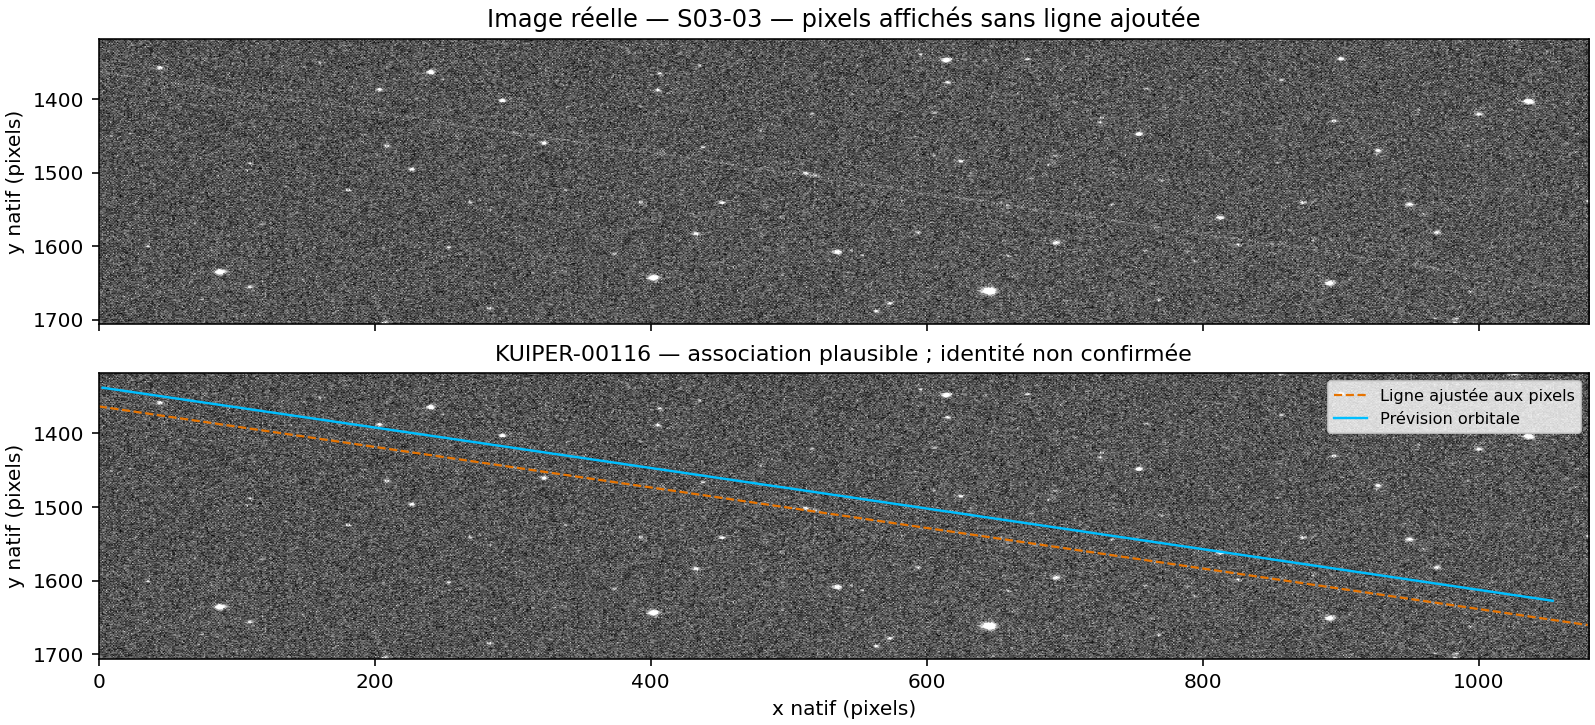
\includegraphics[width=\linewidth]{S03-03-comparison.png}
\caption{S03-03 : vraie image sans annotation en haut ; mesure guidée discontinue et prévision KUIPER-00116 continue en bas. L’orientation concorde approximativement, avec un écart médian de 60,05″. La prévision n’est pas ajustée pour recouvrir la trace.}\label{fig:kuiper}\end{figure}
\begin{figure}[htbp]\centering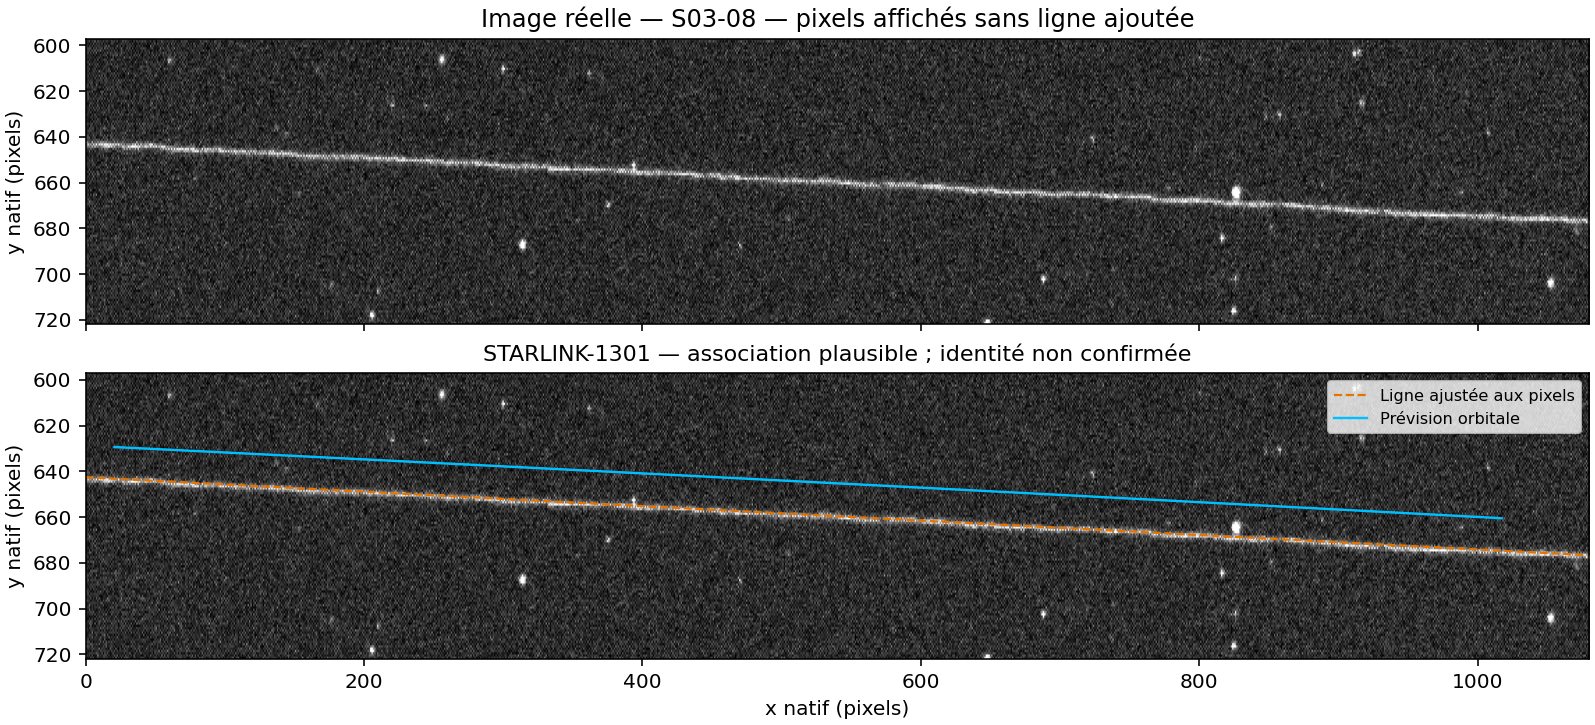
\includegraphics[width=\linewidth]{S03-08-comparison.png}
\caption{S03-08 : même comparaison pour STARLINK-1301, hypothèse plausible. La trace brillante aide la lecture ; elle ne qualifie pas l’heure. Les pixels affichés sont réels ; les lignes sont calculées.}\label{fig:starlink}\end{figure}
\begin{figure}[htbp]\centering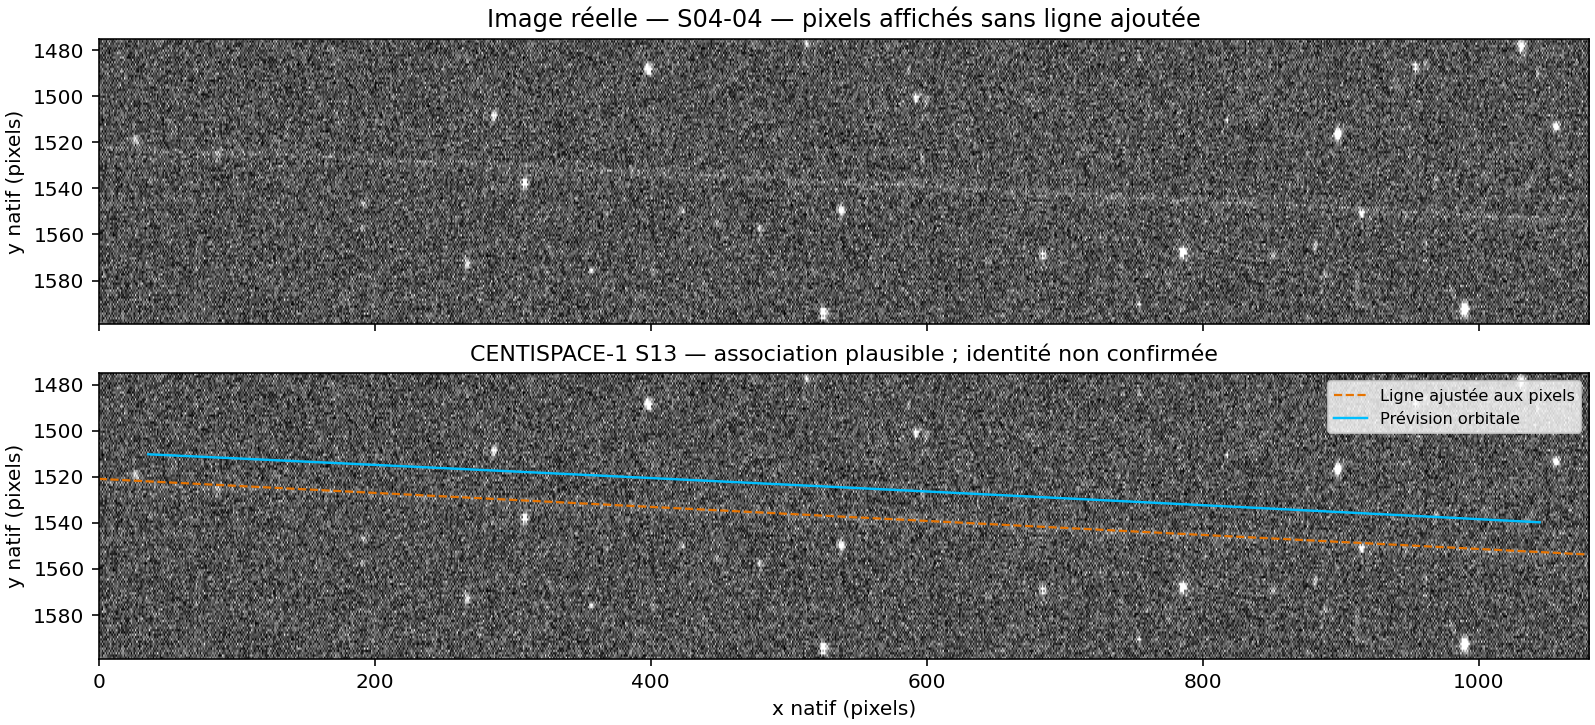
\includegraphics[width=\linewidth]{S04-04-comparison.png}
\caption{S04-04 : même comparaison pour CENTISPACE-1 S13. Ce passage distinct apporte une cohérence supplémentaire, avec le même étalonnage et le même catalogue. Il ne constitue pas un contrôle indépendant ou aveugle.}\label{fig:centi}\end{figure}

Les signaux natifs moyens normalisés et bornés sont respectivement proches de 0,313, 1,831 et 0,298.
Ils dépassent les moyennes des lignes parallèles de contrôle correspondantes.
S04-01 présente un signal de 0,024 et reste faible, douteuse et non identifiée.
Son premier rang numérique, COSMOS 2251 DEB, présente environ 2\,904″ d’écart et 73,6° de différence d’orientation.
Ce rapprochement n’est pas retenu comme association plausible.

Le repérage automatique produit 935 propositions, fortement contaminées par les bords et les résidus stellaires.
Ce nombre ne représente pas 935 satellites.
Les douze autres poses ne présentent pas de trace supplémentaire nette dans cette revue.
Cela ne démontre pas l’absence d’un objet faible ou manqué.
Les essais fictifs de développement restent distincts et ne mesurent pas une efficacité sur la population réelle.

\begin{figure}[htbp]\centering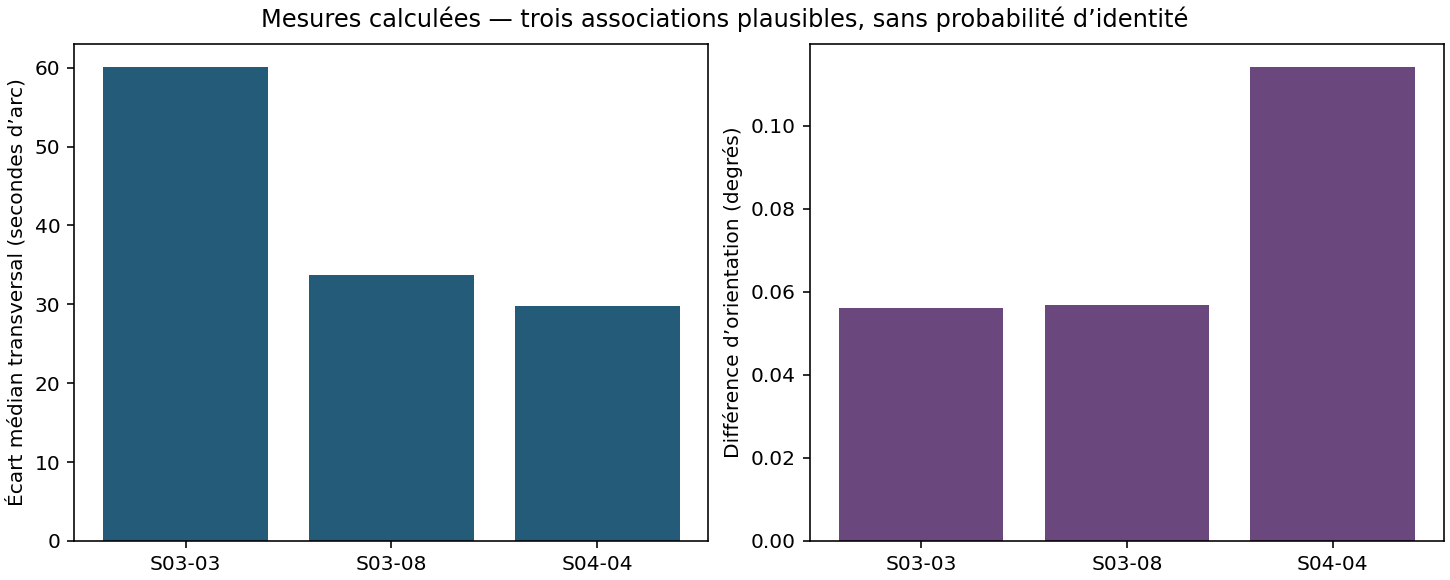
\includegraphics[width=\linewidth]{residuals.png}
\caption{Écarts transversaux médians et différences d’orientation des trois hypothèses. Les barres représentent des valeurs calculées, sans intervalle de confiance ni probabilité d’identité.}\label{fig:residuals}\end{figure}

\subsection{Compatibilité temporelle conditionnelle}
Si $t_a$ et $t_b$ désignent l’entrée et la sortie prévues dans le segment visible, et $E=10$ s, le début de pose peut être compatible avec
\begin{equation}
\Delta_{\mathrm{début}}\in[t_b-E,\ t_a].
\end{equation}
Les temps sont relatifs à DATE-OBS ; $\Delta$ signifie début réel supposé moins date enregistrée.
Les deux passages S03 servent à construire une première intersection.
Le passage S04, déjà examiné, donne un contrôle de cohérence supplémentaire.
L’intersection des trois intervalles est approximativement $[-4,206; +2,029]$ s (figure~\ref{fig:time}).
Ce résultat dépend des identités proposées, de la géométrie et des orbites retenues.
Il ignore des erreurs non quantifiées et ne constitue pas un intervalle de confiance.
Il n’autorise aucune correction automatique des heures.
Si DATE-OBS marquait le milieu ou la fin de pose, l’intervalle serait translaté de cinq ou dix secondes.
Sans référence de temps indépendante, ces conventions restent confondues avec un décalage inconnu.

\begin{figure}[htbp]\centering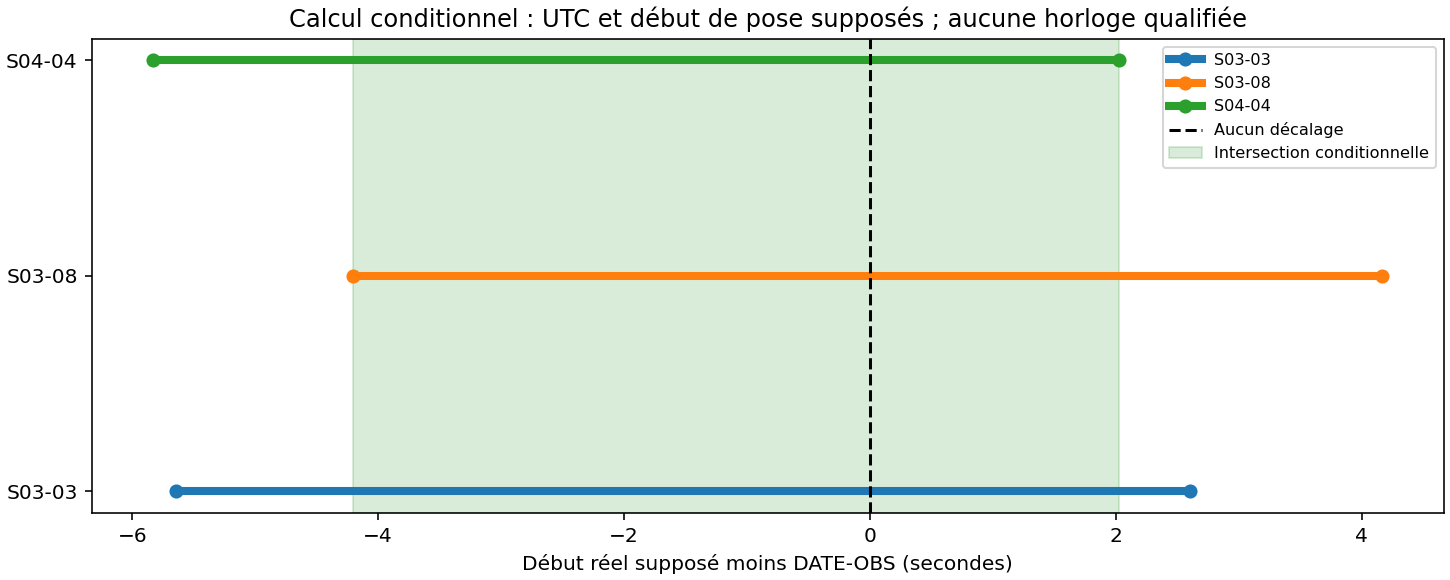
\includegraphics[width=\linewidth]{timing.png}
\caption{Intervalles compatibles sous l’hypothèse UTC et début de pose. L’intersection inclut zéro. Les calculs partagent catalogue et géométrie ; aucune horloge n’est qualifiée.}\label{fig:time}\end{figure}

\section{Discussion et limites}
La concordance des orientations et la proximité spatiale soutiennent trois hypothèses de satellites connus.
Elles ne suffisent pas à certifier les identités : l’incertitude absolue de la carte, le site exact, la hauteur instrumentale, l’horloge et les erreurs orbitales restent à établir.
Aucun seuil probabiliste d’acceptation n’a été calibré sur des faux rapprochements.
La sélection humaine et l’examen préalable de ces cas introduisent un biais.
L’échantillon ne mesure ni taux de récupération, ni taux de faux positifs, ni magnitude limite.
Le classement des jeux disponibles ne garantit pas que tous les objets pertinents figurent dans le catalogue.

La cadence espacée empêche généralement de suivre un même passage rapide dans plusieurs poses.
Une trace tronquée ne fournit pas son instant de début ou sa vitesse par simple division longueur/durée.
La valeur de l’étude réside dans la conservation d’un signal réel, son rapprochement vérifiable et l’exposition des inconnues.
L’absence de correspondance de S04-01 ne constitue pas une indication d’objet nouveau.

Pour progresser, il faudrait qualifier indépendamment le temps et la géométrie, comparer les alternatives et acquérir des passages documentés.
Une mesure de performance demanderait un jeu réservé d’objets réels connus, des témoins et une recherche sans réponses préalables.
Cette étude ne lance pas ces essais et ne reprend pas la fouille de l’archive.

\section{Conclusion}
Seize poses archivées permettent une reproduction guidée de trois associations plausibles avec KUIPER-00116, STARLINK-1301 et CENTISPACE-1 S13.
Une quatrième trace demeure douteuse et non identifiée.
Les résultats montrent l’intérêt d’examiner les archives et de conserver leurs preuves, sans démontrer une capacité générale de détection.
Aucune identification n’est confirmée et aucun nouveau satellite n’est découvert.

\section*{Disponibilité des données et du code}
Le dépôt public est \url{https://github.com/steveprudhomme/gnu-astrophotography-recycle}.
Les seize FITS et leur manifeste sont dans \texttt{examples/data/seestar-series34/}.
Les figures autorisées sont sous CC0-1.0 ; le code est sous GPL-3.0-or-later.
Le journal stable \texttt{JOURNAL-CANDIDATS.md} distingue statut, provenance et historique.
Le guide \texttt{docs/REPRODUIRE-SATELLITES.md} décrit l’installation et les six phases de calcul.
Les classements complets et l’environnement sont dans \texttt{journal/study-results.json}.
Les références tierces sont récupérées séparément et mises en cache avec leurs empreintes.
Un service évolutif peut modifier son catalogue ; le cache historique permet le rejeu exact lorsqu’il est conservé.

\section*{Contributions, assistance et déclarations}
\textbf{Participation citoyenne.} Steve Prud’Homme fournit les observations, formule la question, autorise leur diffusion et demande le journal ainsi que le parcours pédagogique.
Le partage permet à d’autres personnes de reproduire la démarche et de proposer des corrections documentées.
\textbf{Assistance.} Codex a assisté l’analyse, la programmation, la préparation des figures et la rédaction, dont le résumé anglais.
Une assistance par IA ne constitue ni un coauteur ni une validation scientifique indépendante.
Ce manuscrit reste à relire et approuver par l’auteur avant toute soumission à une revue.
\textbf{Financement et conflits.} Aucune déclaration de financement ou de conflit d’intérêts n’a été fournie pour ce manuscrit ; ces renseignements doivent être confirmés avant soumission.
\textbf{Remerciements.} Les projets et services cités rendent possibles les calculs et la comparaison historique.
Aucun endossement par les clubs, l’IAU CPS, les équipes logicielles ou l’UQAM n’est impliqué.

\section*{Note sur les références et l’accessibilité}
Les citations auteur-date et la bibliographie suivent les règles UQAM-APA consultées : ordre alphabétique, initiales, « et » et \textit{et al.} en italique \parencite{uqam}.
Les figures sont décrites par leurs légendes ; le tutoriel fournit des descriptions textuelles plus simples.
Le document ne revendique ni conformité WCAG complète, ni niveau scolaire vérifié.

\clearpage
\printbibliography[title={Références}]
\end{document}
